\documentclass{ximera}
%% handout
%% nohints
%% space
%% newpage
%% numbers

%% You can put user macros here
%% However, you cannot make new environments

\graphicspath{{./}{firstExample/}{secondExample/}}

\usepackage{url}
\usepackage{tikz}
\usepackage{tkz-euclide}
\usetkzobj{all}


\tikzstyle geometryDiagrams=[ultra thick,color=blue!50!black]
\pgfplotsset{compat=1.8}
  \usepackage[T1]{fontenc}
  \usepackage[utf8x]{inputenc} %% we can turn off input when making a master document




\title{Modeling and Predictions}

\begin{document}

\begin{abstract}
We model data as functions and use our models to make predictions.
\end{abstract}
\maketitle

\subsection*{Basic learning objectives}

These are the tasks you should be able to perform with reasonable fluency \textbf{when you arrive at our next class meeting}. Important new vocabulary words are indicated \emph{in italics}. 

\begin{itemize}
	\item Plot points and recognize which type of curve fits the data.
	\item Plot a curve to fit data.
\end{itemize}

\subsection*{Advanced learning objectives}

In addition to mastering the basic objectives, here are the tasks you should be able to perform \textbf{after class, with practice}: 

\begin{itemize}
	\item Use a curve fitted to a table of values to extrapolate values of a function.
    \item Be able to recognize whether a model is a good fit.
    \item Use \href{http://wolframalpha.com}{http://wolframalpha.com} and \href{http://desmos.com}{http://desmos.com} to find curves that fit data.
\end{itemize}

\noindent\hrulefill

In this section we create a model by fitting a curve to data. Then we will use our model to make predictions.

Suppose we are given the function values 
\begin{image}
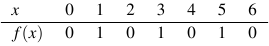
\includegraphics{ModelingTable1.png}
%    \begin{tabular}{llllllll}
%    $x$  & $0$ & $1$ & $2$ & $3$ & $4$ & $5$ & $6$ \\ \hline
%    $f(x)$ & $0$ & $1$ & $0$ & $1$ & $0$ & $1$ & $0$ \\
%    \end{tabular}
\end{image}
Open up \href{http://desmos.com}{http://desmos.com} and create a table containing the data points. A curve that that includes those points must go up and down fairly regularly, so we might try to model the curve with a wave function.

Our first guess is $f(x)=\cos(x)$ which we plot in Desmos. It doesn't work quite right, so we change the function to be $f(x)=a\cos(bx+c)+d$ and create sliders for $a$, $b$, $c$, and $d$. (Follow along by creating this function in Desmos yourself. Otherwise it won't mean anything to you.)


Our function is twice as tall as it needs to be so we set $a=0.5$. The graph needs to be shifted vertically, so that its center line is at $0.5$ so we set $d=0.5$. Our function is too wide so we set $b=2$ or $b=3$ to make it narrower. In fact if we play with it for a minute we might decide $b=\pi$ is a good value. Then we shift things horizontally, and find that $c=\pi$ is a good choice.

Thus our model is $f(x)=0.5\cos(\pi x+\pi)+0.5$. Perhaps another student would have come up with $f(x)=-0.5\cos(\pi x)+0.5$, which happens to be the same curve. 

Is our model a good one? Probably. However, there are many other curves that fit the data.

\begin{question}
Which functions below do not fit the data for the function $f(x)$? (Please don't just guess. You won't learn anything that way.)

\begin{image}
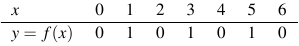
\includegraphics{ModelingTable2.png} 
%    \begin{tabular}{llllllll}
%    $x$  & $0$ & $1$ & $2$ & $3$ & $4$ & $5$ & $6$ \\ \hline
%    $y=f(x)$ & $0$ & $1$ & $0$ & $1$ & $0$ & $1$ & $0$ \\
%    \end{tabular}
\end{image}

    \begin{multipleChoice}
      \choice{$y=\left(\sin(\frac{3\pi}{2}(x))\right)^2$}
      \choice{$y=\big|\left|\mathrm{mod} \left(x-1,2\right)\right|-1\big|$}
      \choice{$y=\left|\sin \left(\frac{\pi x}{2}\right)\right|$}
      \choice{$y=\sin \left(2\pi x\right)-0.5\cos \left(\pi x\right)+0.5$}
      \choice[correct]{$y=\frac{\sin \left(\pi x\right)}{\cos \left(\pi \space x\right)+2}$}
      \choice{$y=\sin \left(\pi \left(x-2.5y\right)\right)$}
    \end{multipleChoice}
    \begin{hint}
    Enter each equation into Desmos. Be careful. You don't need to understand these functions. The purpose of this example is just to show that there might be many curves that fit a single set of data.
    \end{hint}
    \begin{hint}
    You can use \verb|abs(x)| in place of \verb+|x|+ if you are struggling with the absolute value expressions. 
    \end{hint}

\end{question}

\begin{question}
Plot the data in the table
\begin{image}
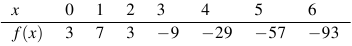
\includegraphics{ModelingTable3.png}
%\begin{tabular}{llllllll}
%    $x$  & $0$ & $1$ & $2$ & $3$  & $4$   & $5$    & $6$   \\ \hline
%    $f(x)$ & $3$ & $7$ & $3$ & $-9$ & $-29$ & $-57$ & $-93$ \\
%\end{tabular}
\end{image}
What is the parent function for the function $f(x)$?

\begin{multipleChoice}
      \choice[correct]{$y=x^2$}
      \choice{$y=x$}
      \choice{$y=x^3$}
      \choice{$y=\sqrt{x}$}
      \choice{$y=\sin(x)$}
      \choice{$y=2^x$}
      \choice{$y=\log(x)$}
\end{multipleChoice}
The formula of the function $f(x)$ is of the form $f(x)=ax^2+bx+c$ for some values $a$, $b$, and $c$. The exact formula $f(x)=$ \answer{-4x^2+8x+3}.
\begin{hint}
The values of $a$, $b$, and $c$ are integers.
\end{hint}

\begin{hint}
Go to \link{http://desmos.com} and create the function $f(x)=ax^2+bx+c$ and use the sliders for $a$, $b$, and $c$ to pinpoint the exact values.
\end{hint}

\end{question}




\begin{question}
Go to \href{https://student.desmos.com}{https://student.desmos.com} and enter the code \verb|vrt3|. Use your real name, and complete the activity (about $15$ minutes.) We will discuss it in class.

The number of pennies in the big circle was \answer{663}.

\end{question}



\end{document}
